% CVPR 2027 submission, first full draft. Rewrite of Neurips_paper_and_rebuttal/paper.tex, with the changes promised in
% Neurips_paper_and_rebuttal/Neurips_rebuttal.tex. Every number traces to CVPR_paper/EXPERIMENT_LOG.md (P-main protocol:
% test-selected checkpoints, calibration hyper-parameters selected cross-fold, never on the target subject).
% \TODO{} marks what is still missing.
\documentclass[10pt,twocolumn,letterpaper]{article}
\usepackage[review]{cvpr}

\usepackage{graphicx}
\usepackage{booktabs}
\usepackage{multirow}
\usepackage{arydshln}
\usepackage{xcolor}
\usepackage{enumitem}
\usepackage{microtype}
% !TeX root = 000main.tex
% needed for compilation in TeXworks 
%\pagestyle{myheadings}

%\usepackage{amsmath,amsfonts,amssymb,rotating}
\usepackage{amssymb,amsmath,amsfonts,epsfig,mdframed,rotating,cancel,mathtools}





\usepackage{bbm}

\usepackage{comment} % To create a block comment



\newcommand{\insertfig}[3]{
\begin{figure}[tbp]\begin{center}\begin{picture}(120,90)
\put(0,-5){\includegraphics[width=12cm,height=9cm,clip=]{#1.eps}}\end{picture}\end{center}
\caption{#2}\label{#3}\end{figure}}

%
\newcommand{\inserttwofig}[4]{
\begin{figure}\begin{center}\begin{picture}(150,170)
\put(10,80){\includegraphics[with=8.5cm]{#1.ps}}
\put(10, 0){\includegraphics[with=8.5cm]{#2.ps}}
\end{picture}\end{center}
\caption{#3}\label{#4}\end{figure}}


%% Commentaires/Discussions
\newcommand{\jc}[1]{{ \color{blue} #1}}
%\newcommand{\jc}[1]{#1}

\newcommand \mqp[1]{{\color{blue}{#1}}}
%\newcommand \mqp[1]{#1}


%% Pour faire des parentheses et crochets corrects plus vite
\renewcommand{\(}{\left(}
\renewcommand{\)}{\right)}
\renewcommand{\[}{\left[}
\renewcommand{\]}{\right]}
\newcommand{\lb}{\llbracket}
%\newcommand{\rb}{\rrbracket}


% bb font symbols
%%new
\def\Q{{\mathbb Q}}
\def\C{{\mathbb C}}
\def\N{{\mathbb N}}
\def\Z{{\mathbb Z}}
\def\R{{\mathbb R}}
\def\E{{\mathbb E}}
\def\F{{\mathbb F}}
\def\P{{\mathbb P}}

%%old
\newfont{\bbb}{msbm10 scaled 500}
\newcommand{\CCC}{\mbox{\bbb C}}

\newfont{\bb}{msbm10 scaled 1100}
\newcommand{\CC}{\mbox{\bb C}}
\newcommand{\RR}{\mbox{\bb R}}
\newcommand{\ZZ}{\mbox{\bb Z}}
\newcommand{\FF}{\mbox{\bb F}}
\newcommand{\GG}{\mbox{\bb G}}
\newcommand{\LL}{\mbox{\bb L}}
\newcommand{\NN}{\mbox{\bb N}}
\newcommand{\PP}{\mbox{\bb P}}
\newcommand{\EE}{\mbox{\bb E}}
 


% Paging
\def\nn{\noindent}


% Math environnement
%\newcommand{\ds}{{\displaystyle}}
\newcommand{\D}{\displaystyle}
\newcommand{\tr}{{^{\triangle}}}

\providecommand{\ie}{{\emph{i.e.}}}


% Math Operator
\DeclareMathOperator{\ind}{1}
\def\i{\perp\!\!\!\perp} % independendent

% Vectors

\newcommand{\av}{{\bf a}}
\newcommand{\bv}{{\bf b}}
\newcommand{\cv}{{\bf c}}
\newcommand{\dv}{{\bf d}}
\newcommand{\ev}{{\bf e}}
\newcommand{\fv}{{\bf f}}
\newcommand{\gv}{{\bf g}}
\newcommand{\hv}{{\bf h}}
\newcommand{\iv}{{\bf i}}
\newcommand{\jv}{{\bf j}}
\newcommand{\kv}{{\bf k}}
\newcommand{\lv}{{\bf l}}
\newcommand{\mv}{{\bf m}}
\newcommand{\nv}{{\bf n}}
\newcommand{\ov}{{\bf o}}
\newcommand{\pv}{{\bf p}}
\newcommand{\qv}{{\bf q}}
\newcommand{\rv}{{\bf r}}
\newcommand{\sv}{{\bf s}}
\newcommand{\tv}{{\bf t}}
\newcommand{\uv}{{\bf u}}
\newcommand{\wv}{{\bf w}}
\newcommand{\vv}{{\bf v}}
\newcommand{\xv}{{\bf x}}
\newcommand{\yv}{{\bf y}}
\newcommand{\zv}{{\bf z}}
\newcommand{\zerov}{{\bf 0}}
\newcommand{\onev}{{\mathbbm 1}}
\newcommand{\Vv}{{\bf V}}   % random vector
\newcommand{\Xv}{{\bf X}}   % random vector
\newcommand{\Yv}{{\bf Y}}   % random vector
\newcommand{\Zv}{{\bf Z}}   % random vector

% Vectors with hat

\newcommand{\avh}{{\bf \hat a}}
\newcommand{\bvh}{{\bf \hat b}}
\newcommand{\cvh}{{\bf \hat c}}
\newcommand{\dvh}{{\bf \hat d}}
\newcommand{\evh}{{\bf \hat e}}
\newcommand{\fvh}{{\bf \hat f}}
\newcommand{\gvh}{{\bf \hat g}}
\newcommand{\hvh}{{\bf \hat h}}
\newcommand{\ivh}{{\bf \hat i}}
\newcommand{\jvh}{{\bf \hat j}}
\newcommand{\kvh}{{\bf \hat k}}
\newcommand{\lvh}{{\bf \hat l}}
\newcommand{\mvh}{{\bf \hat m}}
\newcommand{\nvh}{{\bf \hat n}}
\newcommand{\ovh}{{\bf \hat o}}
\newcommand{\pvh}{{\bf \hat p}}
\newcommand{\qvh}{{\bf \hat q}}
\newcommand{\rvh}{{\bf \hat r}}
\newcommand{\svh}{{\bf \hat s}}
\newcommand{\tvh}{{\bf \hat t}}
\newcommand{\uvh}{{\bf \hat u}}
\newcommand{\wvh}{{\bf \hat w}}
\newcommand{\vvh}{{\bf \hat v}}
\newcommand{\xvh}{{\bf \hat x}}
\newcommand{\yvh}{{\bf \hat y}}
\newcommand{\zvh}{{\bf \hat z}}
\newcommand{\zerovh}{{\bf \hat 0}}
\newcommand{\onevh}{{\bf \hat 1}}

% Matrices

\newcommand{\Am}{{\bf A}}
\newcommand{\Bm}{{\bf B}}
\newcommand{\Cm}{{\bf C}}
\newcommand{\Dm}{{\bf D}}
\newcommand{\Em}{{\bf E}}
\newcommand{\Fm}{{\bf F}}
\newcommand{\Gm}{{\bf G}}
\newcommand{\Hm}{{\bf H}}
\newcommand{\Id}{{\bf I}}
\newcommand{\Jm}{{\bf J}}
\newcommand{\Km}{{\bf K}}
\newcommand{\Lm}{{\bf L}}
\newcommand{\Mm}{{\bf M}}
\newcommand{\Nm}{{\bf N}}
\newcommand{\Om}{{\bf O}}
\newcommand{\Pm}{{\bf P}}
\newcommand{\Qm}{{\bf Q}}
\newcommand{\Rm}{{\bf R}}
\newcommand{\Sm}{{\bf S}}
\newcommand{\Tm}{{\bf T}}
\newcommand{\Um}{{\bf U}}
\newcommand{\Wm}{{\bf W}}
\newcommand{\Vm}{{\bf V}}
\newcommand{\Xm}{{\bf X}}
\newcommand{\Ym}{{\bf Y}}
\newcommand{\Zm}{{\bf Z}}
\newcommand{\Sigm}{{\bf \Sigma}}

% Calligraphic

\newcommand{\Ac}{{\cal A}}
\newcommand{\Bc}{{\cal B}}
\newcommand{\Cc}{{\cal C}}
\newcommand{\Dc}{{\cal D}}
\newcommand{\Ec}{{\cal E}}
\newcommand{\Fc}{{\cal F}}
\newcommand{\Gc}{{\cal G}}
\newcommand{\Hc}{{\cal H}}
\newcommand{\Ic}{{\cal I}}
\newcommand{\Jc}{{\cal J}}
\newcommand{\Kc}{{\cal K}}
\newcommand{\Lc}{{\cal L}}
\newcommand{\Mc}{{\cal M}}
\newcommand{\Nc}{{\cal N}}
\newcommand{\Oc}{{\cal O}}
\newcommand{\Pc}{{\cal P}}
\newcommand{\Qc}{{\cal Q}}
\newcommand{\Rc}{{\cal R}}
\newcommand{\Sc}{{\cal S}}
\newcommand{\Tc}{{\cal T}}
\newcommand{\Uc}{{\cal U}}
\newcommand{\Wc}{{\cal W}}
\newcommand{\Vc}{{\cal V}}
\newcommand{\Xc}{{\cal X}}
\newcommand{\Yc}{{\cal Y}}
\newcommand{\Zc}{{\cal Z}}

% Bold greek letters
% for non italic greek letters use package \usepackage{upgreek} and \boldsymbol\uptheta

\newcommand{\alphav}{\hbox{\boldmath$\alpha$}}
\newcommand{\betav}{\hbox{\boldmath$\beta$}}
\newcommand{\gammav}{\hbox{\boldmath$\gamma$}}
\newcommand{\deltav}{\hbox{\boldmath$\delta$}}
\newcommand{\etav}{\hbox{\boldmath$\eta$}}
\newcommand{\lambdav}{\hbox{\boldmath$\lambda$}}
\newcommand{\epsilonv}{\hbox{\boldmath$\epsilon$}}
\newcommand{\nuv}{\hbox{\boldmath$\nu$}}
\newcommand{\muv}{\hbox{\boldmath$\mu$}}
\newcommand{\zetav}{\hbox{\boldmath$\zeta$}}
\newcommand{\phiv}{\hbox{\boldmath$\phi$}}
\newcommand{\psiv}{\hbox{\boldmath$\psi$}}
\newcommand{\thetav}{\hbox{\boldmath$\theta$}}
\newcommand{\tauv}{\hbox{\boldmath$\tau$}}
\newcommand{\omegav}{\hbox{\boldmath$\omega$}}
\newcommand{\xiv}{\hbox{\boldmath$\xi$}}
\newcommand{\sigmav}{\hbox{\boldmath$\sigma$}}
\newcommand{\piv}{\hbox{\boldmath$\pi$}}
\newcommand{\rhov}{\hbox{\boldmath$\rho$}}

\newcommand{\Gammam}{\hbox{\boldmath$\Gamma$}}
\newcommand{\Lambdam}{\hbox{\boldmath$\Lambda$}}
\newcommand{\Deltam}{\hbox{\boldmath$\Delta$}}
\newcommand{\Sigmam}{\hbox{\boldmath$\Sigma$}}
\newcommand{\Phim}{\hbox{\boldmath$\Phi$}}
\newcommand{\Pim}{\hbox{\boldmath$\Pi$}}
\newcommand{\Psim}{\hbox{\boldmath$\Psi$}}
\newcommand{\Thetam}{\hbox{\boldmath$\Theta$}}
\newcommand{\Omegam}{\hbox{\boldmath$\Omega$}}
\newcommand{\Xim}{\hbox{\boldmath$\Xi$}}

% intercomm notation

\newcommand{\js}{(j^*)}%previous request
\renewcommand{\j}{(j)}%one arbitrary previous request
\renewcommand{\k}{(k)}%one arbitrary current request
\renewcommand{\l}{(l)}%current request
\renewcommand{\L}{(L)}%current request
\newcommand{\Ejs}{\Ec^*}%{\Ec_{j^*}}%set

\newcommand{\jm}{{(j_{m})}}% source indices of the true previous request in the set


\newcommand{\jms}{{j_{m^*}}}% indices of the true previous request in the set

%\newcommand{\Xset}{\mathcal{X}}%set of source
\newcommand{\Xl}{X_{(l)}}%arbitrary source
\newcommand{\Xone}{X_{(1)}}% first source
\newcommand{\Xk}{X_{(k)}}%requested source
\newcommand{\Xjs}{X_{(j^*)}}%previous requested source
\newcommand{\Xj}{X_{(j)}}% arbitrary previous source
\newcommand{\XJk}{X_{(J_{\k})}}% arbitrary previous source
\newcommand{\Xjone}{X_{(j_1)}}% first possible previously requested source
\newcommand{\XjM}{X_{(j_M)}}% last possible previously requested source
\newcommand{\XjMk}{X_{({j_M}_{\tiny (k)})}}% last possible previously requested source
\newcommand{\Xjm}{X_{(j_m)}}% arbitrary possible previously requested source


\newcommand{\Jsetk}{\mathcal{J}_{(k)}}%possible set of previous requested sources 
\newcommand{\Jsetkd}{\mathcal{\widetilde{J}}_{(k)}}%possible set of previous requested sources (lossy case)

\newcommand{\Mk}{M_{(k)}}%Number of possible previous requests (either  number of possible indicies or number of possible set of indices)
\newcommand{\M}{M}%Number of possible previous requests (either  number of possible indicies or number of possible set of indices)
\newcommand{\Ssetl}{\mathcal{S}_{(l)}}%possible set of previous requested sources 
\newcommand{\Rkjs}{R_{(k)|(j^*)}}%rate
\newcommand{\RkEjs}{R_{(k)|\Ec^*}}%rate
\newcommand{\Ffamk}{\mathcal{F}_{(k)}}% family of subset of possible previous requested sources
\newcommand{\sigA}{\pi}	% Ordering application
\newcommand{\Sk}{S_{(k)}}%storage

\newcommand{\Pset}{\mathscr{P}}
\newcommand{\Ppmf}{\mathcal{P}}

\newcommand{\xJxj}{_{\xv^n,\xv_{\j}^n}}  % fro the types
\newcommand{\xxj}{_{\xv^n|\xv_{\j}^n}}
\newcommand{\xxjs}{_{\xv^n|\xv_{\js}^n}}

\newcommand{\xkJxj}{_{\xv_{\k}^n,\xv_{\j}^n}}
\newcommand{\xkxj}{_{\xv_{\k}^n|\xv_{\j}^n}}
\newcommand{\xkxjs}{_{\xv_{\k}^n|\xv_{\js}^n}}


% Unknown statistics, non iid case
\newcommand{\SetET}{\boldsymbol{\hat{\theta}}^{(u_n)}}
\newcommand{\SetETR}{\boldsymbol{\widehat{\Theta}}^{(u_n)}}
\newcommand{\SetE}{\boldsymbol{\hat{\theta}}}
\newcommand{\SetER}{\boldsymbol{\widehat{\Theta}}}
\newcommand{\An}{A_{n}(\mathbf{X}^{n},\Xv_{\j}^{n})}
\newcommand{\Bn}{B_{n}(\mathbf{X}^{n},\Xv_{\j}^{n})}
\newcommand{\Vn}{V_{n}(\mathbf{X}^{n},\Xv_{\j}^{n})}
\newcommand{\Anx}{A_{n}(\mathbf{x}^{n},\xv_{\j}^{n})}
\newcommand{\Bnx}{B_{n}(\mathbf{x}^{n},\xv_{\j}^{n})}
\newcommand{\Vnx}{V_{n}(\mathbf{x}^{n},\xv_{\j}^{n})}
\newcommand{\Pt}{Q}
\newcommand{\pt}{q}

% to remove: no more used
\newcommand{\Fk}{F_{(k)}}%Number of family of subset of possible previous requested sources 
\newcommand{\Jk}{J_{(k)}}%Number of possible set of previous requested sources 



\newcommand{\tp}{\theta}
\newcommand{\Tp}{\Theta}
\newcommand{\Etp}{\mathcal{T}}
\newcommand{\tpe}{\hat{\theta}}
\newcommand{\Hs}{\overline{H}}
\newcommand{\plim}{\text{p}\text{ - }\underset{n\rightarrow \infty}{\lim\sup}~}
\newcommand{\prlim}{\text{p}\text{ -}\underset{n\rightarrow \infty}{\lim}~}

\newcommand{\sigx}{\sigma_k}
\newcommand{\sigy}{\sigma_j}
\newcommand{\cc}{\rho_{k,j}}
\newcommand{\Ckj}{\Sigma_{(k,j)}}
\newcommand{\sigkj}{\sigma_{k,j}}
\newcommand{\sigkjs}{\sigma_{k,j^{*}}}
\newcommand{\Un}{\mathbf{U}^n}
\newcommand{\un}{\mathbf{u}^n}

\newcommand{\Reqset}{\mathcal{K}} % the request set
\newcommand{\Reqvec}{\mathbf{K}} % the request vec
\newcommand{\NReq}{K} % the number of request 
\newcommand{\reqZero}{(k_0)} % the first request index
\newcommand{\reqOne}{(k_1)} % the first request index
\newcommand{\reqNReq}{(k_{\NReq})} % the Kth request index
\newcommand{\reqt}{(k_t)} % the t-th request index
\newcommand{\reqtprev}{(k_{t-1})} % the t-1-th request index

\newcommand{\G}{\mathcal{G}} % the graph
\newcommand{\V}{\mathcal{V}} % the graph
%\newcommand{\Edge}{\mathcal{E}} % the graph


% mixed symbols

\newcommand{\sinc}{{\hbox{sinc}}}
\newcommand{\diag}{{\hbox{diag}}}
\renewcommand{\det}{{\hbox{det}}}
\newcommand{\trace}{{\hbox{tr}}}
\newcommand{\sign}{{\hbox{sign}}}
\renewcommand{\arg}{{\hbox{\rm arg}}}
\newcommand{\var}{{\hbox{var}}}
\newcommand{\SINR}{\hbox{SINR}}
\newcommand{\SNR}{\hbox{SNR}}
\newcommand{\Ei}{{\rm E}_{\rm i}}
\renewcommand{\Re}{{\rm Re}}
\renewcommand{\Im}{{\rm Im}}
%\newcommand{\eqdef}{\stackrel{\Delta}{=}}
% use \triangleq instead in amsmath amssymb
\newcommand{\eqe}{\stackrel{.}{=}}
\newcommand{\<}{\left\langle}
\renewcommand{\>}{\right\rangle}
\newcommand{\smaller}{\negthickspace > \negthickspace}
\newcommand{\bit}{\mbox{ bit }}
\newcommand{\bits}{\mbox{ bits }}
\newcommand{\ifm}{\mbox{ if }}
\newcommand{\SW}{{\rm SW}}
\newcommand{\Ca}{{\rm C}}
\newcommand{\qqquad}{\qquad \quad}

\newcommand{\setN}{\{1,\,\ldots,\, N\}}
\newcommand{\setM}{\{1,\,\ldots,\, M\}}
\newcommand{\setK}{\{1,\,\ldots,\, K\}}
% math symbol

\def\<{\langle}
\def\>{\rangle}
\newcommand{\foralls}{\forall \ }
\newcommand{\indep}{\quad \begin{rotate}{90}{$\models$}\end{rotate} \quad}


\newcommand{\conv}{\ensuremath{\operatorname{conv}}}
\newcommand{\vol}{\ensuremath{\operatorname{vol}}}
\newcommand{\cut}{\ensuremath{\operatorname{cut}}}
\newcommand{\ncut}{\ensuremath{\operatorname{Ncut}}}
\newcommand{\assoc}{\ensuremath{\operatorname{assoc}}}
\newcommand{\nassoc}{\ensuremath{\operatorname{Nassoc}}}
%\newcommand{\I}{\ensuremath{\operatorname{\textbf{I}}}}

\newcommand{\I}{{\bf I}}


\newcommand{\Diag}{\ensuremath{\operatorname{Diag}}}
\newcommand{\cost}{\ensuremath{\operatorname{cost}}}

\DeclareMathOperator{\Tr}{Tr}
\DeclareMathOperator{\amin}{argmin}
%\newcommand{\sign}{\ensuremath{\operatorname{sign}}}
\newcommand{\minimize}[2]{\underset{{#1}}{\text{minimize}}\;{#2}}
\newcommand{\argmin}[1]{\underset{{#1}}{\text{argmin}}}
\newcommand{\argmax}[1]{\underset{{#1}}{\text{argmax}}}
\newcommand{\dom}{\ensuremath{\mathrm{dom}\,}}
\newcommand{\rank}{\ensuremath{\mathrm{rank}\,}}
\newcommand{\sri}{\ensuremath{\mathrm{sri}\,}}
\newcommand{\ri}{\ensuremath{\mathrm{ri}\,}}
%\newcommand{\Id}{\ensuremath{\mathrm{Id}}}
\newcommand{\prox}{\ensuremath{\operatorname{prox}}}
\newcommand{\proj}{\ensuremath{\operatorname{proj}}}
\newcommand{\fastMU}{\ensuremath{\operatorname{fastMU}}}



% ----- new macros 
\newcommand{\fid}{\ensuremath{\operatorname{fid}}}
\newcommand{\prior}{\ensuremath{\operatorname{prior}}}

\newcommand{\Jfid}{J_{\mathrm{fid}}}
\newcommand{\Jprior}{J_{\mathrm{prior}}}

\newcommand{\thetaG}{\thetav_\Gamma}
\newcommand{\thetaC}{\thetav_C}

\newcommand{\Gammatheta}{\Gamma_{\thetav_\Gamma}}
\newcommand{\Ctheta}{C_{\thetav_C}}  
\newcommand{\Phitheta}{\Phi_{\thetav_\Phi}}  
\newcommand{\Rtheta}{R_{\thetav_R}}  

\newcommand{\Ttheta}{T_{\thetav}}
\newcommand{\gphi}{g_{\phiv}}

\newcommand{\loss}{\mathcal{L}}
\newcommand{\losstraj}{\mathcal{L}_{\mathrm{traj}}}
\newcommand{\lossfinal}{\mathcal{L}_{\mathrm{final}}}
\newcommand{\losssmooth}{\mathcal{L}_{\mathrm{smooth}}}
\newcommand{\lossstep}{\mathcal{L}_{\mathrm{step}}}





% ----------

\newcommand{\fastMUmin}{\ensuremath{\operatorname{fastMUmin}}}
\newcommand{\MU}{\ensuremath{\operatorname{MU}}}
\newcommand{\kmax}{\ensuremath{K_\text{max}}}



\DeclarePairedDelimiter\ceil{\lceil}{\rceil}
\DeclarePairedDelimiter\floor{\lfloor}{\rfloor}

 		



%\renewenvironment{proof}{\textbf{Proof}}{\qed}

%%% tikz for graph 

\usepackage{tikz,tkz-tab}

\usetikzlibrary{fit,automata,positioning,calc,shapes}
\usepackage{ifthen}

\ifdefined\circlenode
\else
\newcommand{\circlenode}[3]{
	\node [draw, circle, inner sep=2pt, #1] (#2) {#3};
}
\fi
\ifdefined\sqnode
\else
\newcommand{\sqnode}[3]{
	\node [draw, rectangle, inner sep=2pt, #1] (#2) {#3};
}
\fi



%%% index

\newcommand{\iopt}{\overline{i}}
\newcommand{\jopt}{\overline{j}}
\newcommand{\topt}{\overline{t}}
%\usepackage{amsthm} % Load theorem package

 

%%%%% color definition 
\definecolor{darkgreen}{rgb}{0.1,0.5,0}
\definecolor{Midnightblue}{rgb}{.2,.2,.7}
\definecolor{mypink3}{cmyk}{0, 0.7808, 0.4429, 0.1412}

\def\blue#1{\textcolor{Midnightblue}{#1}}

\def\bblue#1{\textbf{\textcolor{Midnightblue}{#1}}}

\definecolor{amber}{rgb}{1.0, 0.49, 0.0}

\def\oran#1{\textcolor{amber}{#1}}

\def\redm#1{\textcolor{mypink3}{#1}}

\def\boran#1{\textbf{\textcolor{amber}{#1}}}
\def\green#1{\textcolor{darkgreen}{#1}}


% remove/comment the sentence 

\newcommand \remove[1]{ }

 




 


\newcommand{\TODO}[1]{\textbf{\color{red}[TODO: #1]}}

\definecolor{cvprblue}{rgb}{0.21,0.49,0.74}
\usepackage[pagebackref,breaklinks,colorlinks,allcolors=cvprblue]{hyperref}

\def\confName{CVPR}
\def\confYear{2027}

\title{Mind the Accuracy Gap: Label-Free Subject Calibration\\for EEG-to-Image Decoding}

\author{Anonymous CVPR submission}

\begin{document}
\maketitle

%=====================================================================
\begin{abstract}
Neural decoding of visual experience from electroencephalography (EEG) has achieved strong performance in intra-subject settings, but current methods fail to generalize across individuals. On the standard 200-way benchmark, top-1 accuracy drops from above 80\% within subjects to around 35\% for an unseen subject. A decoder deployed for a new user, however, always knows its candidate images, as the zero-shot benchmark already assumes, and continuously receives unlabeled signal from that user. We formalize this setting as \emph{label-free transductive subject calibration}, make explicit the assumptions it rests on, and propose an evaluation protocol with four test regimes, model selection rules that never access the target subject, and per-subject reporting. Within this protocol, we introduce \textbf{SAGE} (\textbf{S}ubject-\textbf{A}gnostic \textbf{G}eometrically-aligned \textbf{E}mbeddings), which registers the unlabeled EEG point cloud onto the candidate images through shrinkage whitening, hubness correction and iterated Sinkhorn--Procrustes alignment. On the standard transductive test of THINGS-EEG-2, SAGE raises cross-subject top-1 accuracy from 35.8\% to 84.6\%, against 66.5\% for the strongest prior label-free method, and improves on it for every subject of each of the ten encoders we test. We further show that the one-to-one structure of the test set alone accounts for the accuracy of prior methods, that SAGE matches a supervised alignment fitted on the entire labeled training session of the new subject, and that the benefit of calibration is predicted by the agreement between the similarity structures of the EEG and image embeddings rather than by zero-shot accuracy; aligning the encoder to the final layer of the image model, a common choice, removes most of it. We quantify eight evaluation pitfalls, including the regimes in which transductive calibration, ours included, falls below the uncalibrated decoder.
\end{abstract}

%=====================================================================
\section{Introduction}
\label{sec:intro}

Decoding visual perception from brain activity is a central goal of neuroscience~\cite{kamitani2005decoding,carlson2013representational,grootswagers2017decoding}, with applications ranging from the study of visual representations~\cite{cichy2014resolving,contini2017decoding} to assistive brain-computer interfaces~\cite{lawhern2018eegnet,gao2021interface}. EEG is especially attractive for this problem because it is non-invasive, has high temporal resolution, and is relatively inexpensive. In the now-standard \emph{EEG-to-image retrieval} setting~\cite{spampinato2017deep,gifford2022things,grootswagers2022things}, both EEG signals and images are represented in a joint embedding space, and retrieval is performed by selecting, for a given EEG signal, the closest image from a candidate set. Since related progress in \emph{fMRI}-to-image reconstruction further suggests that neural decoding can benefit strongly from well-structured latent spaces and powerful visual priors~\cite{takagi2023highres,ozcelik2023natural,scotti2023mindeye,scotti2024mindeye2}, recent work has largely focused on contrastive alignment between EEG embeddings and features from large pre-trained vision models~\cite{song2024nice,li2024atm,wu2025ubp,zhang2025neurobridge,du2025shallow}. With progressively stronger EEG encoders and image targets, these methods now exceed 80\% top-1 accuracy in the standard \emph{intra-subject} 200-way retrieval setting~\cite{du2025shallow}. In the \emph{cross-subject} setting, however, where the encoder must generalize to a held-out subject, accuracy remains far lower under the leave-one-subject-out (LOSO) protocol, between 20\% and 35\% for the strongest published encoders~\cite{du2025shallow,zhang2025neurobridge,yadav2026svtl}.

\begin{figure*}[t]
  \centering
  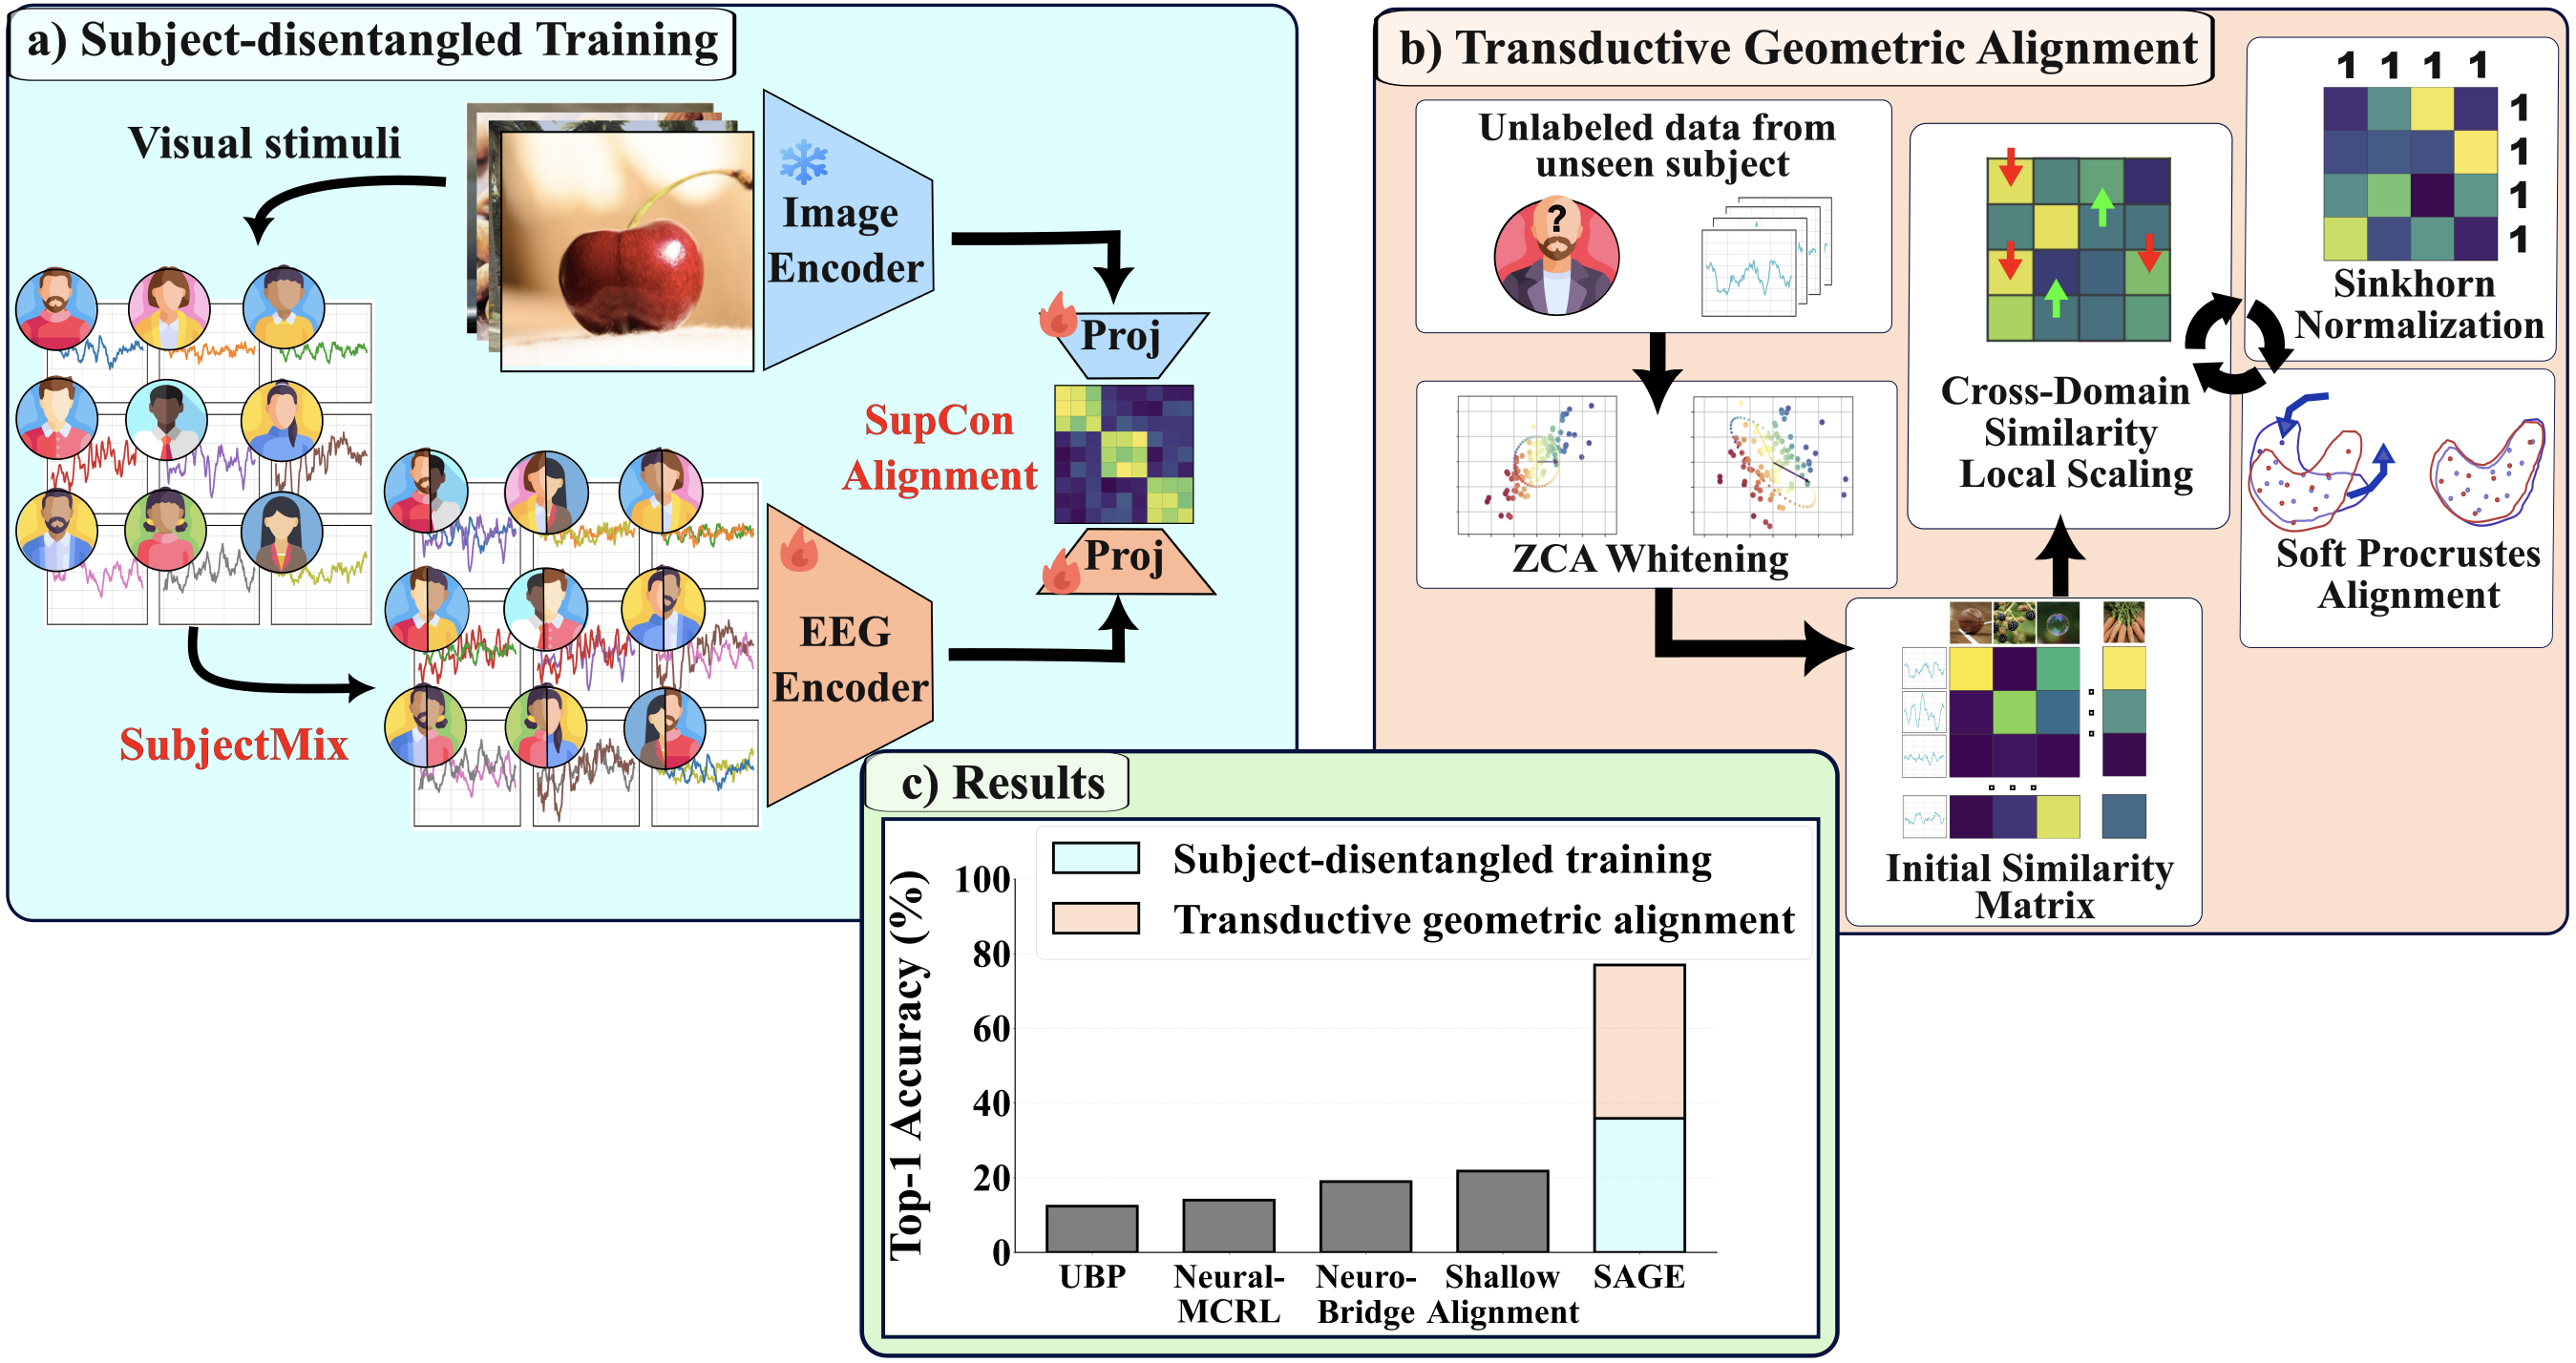
\includegraphics[width=0.92\textwidth]{figures/pipeline.png}
  \caption{Overview of the SAGE pipeline.
  a) The base encoder is trained on stimulus-grouped batches with cross-subject mixing of same-stimulus EEG.
  b) At test time, the calibration corrects the subject-specific misalignment of the unlabeled EEG embeddings through whitening, local scaling and an iterative Sinkhorn--Procrustes refinement.
  c) Top-1 accuracy of the zero-shot encoder and after transductive calibration, which requires the known candidate set.
  \TODO{Redraw panel (c) with the current numbers (zero-shot 35.8, SCORE 66.5, SAGE 84.6) and mark the calibrated bars as transductive, as promised in the rebuttal.}}
  \label{fig:pipeline}
\end{figure*}

This gap is rooted in the characteristic inter-subject variability of EEG. Scalp recordings are subject-specific mixtures of underlying neural sources: skull geometry, cortical folding, and electrode placement induce a different spatial mixing matrix for each individual~\cite{onton2006imaging}. Inter-subject differences in covariance structure and spatial filtering further amplify this mismatch~\cite{blankertz2008optimizing,barachant2010riemannian,samek2013transferring,haufe2014interpretation}. How these differences produce the loss of accuracy on a new subject remains open: a recent survey reviews the mechanisms and mitigation strategies proposed for the cross-subject gap without settling on one~\cite{li2026crosssubject}, and subject identity has been shown to persist in representations trained to be transferable~\cite{lin2026identitytrap}. We take no position on the origin of the gap. We study a correction, estimated from unlabeled data, that recovers part of it, and treat its success as a property of the correction rather than as evidence about the cause.

Benchmarks currently measure only the two extremes of the adaptation spectrum: a zero-shot decoder that sees nothing of the new subject, and an intra-subject decoder trained on hours of labeled recordings. A deployed decoder sits between the two. It knows its candidate set, as the zero-shot benchmark already assumes, and continuously receives unlabeled signal from its user, but no labels. Classical BCI routinely exploits such unlabeled data, through unsupervised re-centering of the target covariance structure~\cite{zanini2018transfer,he2020euclidean,rodrigues2019rpa} or through the known structure of the stimulation paradigm~\cite{kindermans2012bayesian,huebner2017learning}. EEG-to-image retrieval offers a stronger handle than either: the candidate images form a second point cloud, so the unlabeled target embeddings can be aligned \emph{across modalities} to the known stimuli rather than to themselves. Three recent methods do this~\cite{huang2026sattc,cui2026score,yadav2026svtl}. Each, however, evaluates in its own regime and with its own model selection rule, and none states what its test-time procedure assumes about the unlabeled data, so their numbers are not comparable and their failure modes are unknown.

Accordingly, we distinguish two operating modes throughout the paper. \emph{Zero-shot} denotes the inductive cross-subject encoder evaluated without any test-time adaptation; its results are claims about cross-subject decoding in general. \emph{Calibrated} denotes a transductive procedure that acts on the unlabeled queries of the held-out subject and the candidate image set taken jointly; its results apply only to that setting, and we state for each regime what it assumes about the queries. Our contributions are summarized as follows:
\begin{enumerate}[leftmargin=1.3em,itemsep=1pt,topsep=2pt]
  \item \textbf{A setting and a protocol.}
    We formalize calibration from unlabeled target data and a known gallery, name the four assumptions that existing evaluations leave implicit, and define four test regimes, from the standard bijective test to streams, partial coverage and open galleries, together with selection rules that never touch the target subject.
  \item \textbf{Transductive geometric alignment.}
    We reframe calibration as a point-cloud registration problem~\cite{besl1992method,grave2019wasserstein}: given the unlabeled EEG queries and the candidate images, SAGE estimates a subject-specific orthogonal correction by alternating Sinkhorn correspondence estimation~\cite{cuturi2013sinkhorn} and Procrustes alignment~\cite{schonemann1966procrustes}, after shrinkage whitening and CSLS~\cite{conneau2018muse}. A single budget-dependent damping makes the same procedure safe on short streams. On THINGS-EEG-2, SAGE reaches 84.6\% top-1 across three training seeds, against 66.5\% for the strongest prior label-free method, without using any labeled test data.
  \item \textbf{What the gain is made of.}
    We show that decoding the uncalibrated scores with a one-to-one assignment, without any adaptation, already reaches 66.2\%, the accuracy of prior methods. SAGE adds 18 points on top of this correspondence prior, matches a supervised rotation fitted on 16{,}540 labeled pairs from the new subject, and its gain grows with the signal-to-noise ratio of the queries rather than with the weakness of the base decoder. Across ten encoders and fourteen training variants, the gain follows the representational similarity between EEG and image embeddings~\cite{kriegeskorte2008rsa}, and it depends strongly on the layer of the image model used as target.
  \item \textbf{Pitfalls.}
    We quantify eight evaluation pitfalls on our own pipeline. Among them, the bijection that the standard test provides is the source of most of the calibration gain, and the same calibration falls below the zero-shot decoder when only part of the gallery is queried or when distractor images are added. A label-free estimate of the candidates actually present brings SAGE back to the level of SCORE in both cases.
\end{enumerate}
The full training and evaluation code, the configuration files for every reported run, and the trained checkpoints will be released publicly.

%=====================================================================
\section{Related Work}
\label{sec:related}

\paragraph{EEG-to-image decoding.}
Visual neural decoding has progressed from early supervised, subject-specific classifiers on labeled EEG-image pairs~\cite{spampinato2017deep} and tripartite multimodal alignment frameworks~\cite{du2023bravl} to a zero-shot retrieval paradigm enabled by large-scale serial visual presentation benchmarks~\cite{gifford2022things,grootswagers2022things}.
NICE~\cite{song2024nice} established the contrastive alignment framework, using an InfoNCE~\cite{oord2019cpc} objective to align TSConv EEG embeddings with frozen CLIP~\cite{radford2021clip} image features.
Subsequent work tackled the \emph{perceptual fidelity gap} between rich visual stimuli and noisy brain responses: UBP~\cite{wu2025ubp} dynamically blurs image targets proportional to stimulus uncertainty, while NeuroBridge~\cite{zhang2025neurobridge} introduced principled image augmentation for better bidirectional alignment.
ENIGMA~\cite{kneeland2025enigma} further demonstrated efficient multi-subject adaptation in a few-shot setting through subject-specific latent layers coupled with a compact bottleneck.
Shallow Alignment~\cite{du2025shallow} showed that extracting intermediate-layer features from large pretrained vision models~\cite{chen2024internvl} yields a better granularity matching between EEG and image, achieving 82.6\% intra-subject and 21.8\% cross-subject top-1 accuracy.
We adopt Shallow Alignment's image representation strategy for our base encoders. These works improve the inductive encoder; we leave the encoder frozen and study what can be recovered at test time.

\paragraph{Cross-subject generalization.}
Inter-subject EEG variability, rooted in anatomical differences, non-stationarities, and individual neural coding strategies~\cite{jayaram2016transfer,lotte2018review,samek2013transferring,onton2006imaging}, has long been identified as the central bottleneck for generalizable BCI systems.
In the EEG-to-image retrieval setting, this produces a stark capacity gap: intra-subject top-1 accuracy exceeds 80\%, while cross-subject accuracy remains around 20\%~\cite{du2025shallow,zhang2025neurobridge}.
Training-time approaches such as adversarial inference~\cite{ozdenizci2020adversarial} and multi-source distribution matching~\cite{chen2021msmda,she2023multisource} have been shown to improve robustness for paradigm-specific encoders, but do not provide a label-free test-time correction to adapt to new subjects. At test time, Riemannian re-centering~\cite{zanini2018transfer}, Euclidean alignment~\cite{he2020euclidean} and Riemannian Procrustes analysis~\cite{rodrigues2019rpa} align a new subject's covariance structure without labels, and ERP spellers learn from the known proportions of target and non-target stimuli~\cite{kindermans2012bayesian,huebner2017learning}, the closest classical analogue to calibration from a known candidate set. These methods align the target to itself or to source statistics; in retrieval, the gallery provides a second, fixed point cloud in the embedding space, which they do not use.
Large EEG datasets and pretrained encoders have also motivated \emph{EEG foundation models} aimed at transferable representations~\cite{elouahidi2025reve,cui2023neurogpt}, but these primarily address within-modality prediction and subject transfer in EEG, not alignment between neural signals and a visual embedding space.

\paragraph{Label-free calibration for EEG-to-image retrieval.}
SATTC~\cite{huang2026sattc} combines subject-adaptive whitening with adaptive local scaling and a structural expert, and reports an improvement from 9.2\% to 14.8\% top-1 on top of ATM. SCORE~\cite{cui2026score} observes that subjects preserve concept relationships along different coordinate directions, trains the encoder on simulated recovery episodes, and at deployment estimates one orthogonal map from hubness-corrected mutual nearest neighbours, reaching 53.2\%. Concurrently, SVTL~\cite{yadav2026svtl} applies a similar training-free refinement to a structured visual target and reaches 48.1\%. All three are transductive in the target data and rely on the one-to-one structure of the 200-image test, yet none states this, and each selects its checkpoint on the test subject.

\paragraph{Transductive inference and test-time adaptation.}
Test-time adaptation updates normalization statistics or parameters on unlabeled target batches~\cite{li2018adabn,wang2021tent,liang2020shot,iwasawa2021t3a}, and transductive vision-language methods exploit the joint structure of a query batch~\cite{martin2024transductive,zanella2024transclip}. Evaluations of these methods have repeatedly shown that gains measured on curated test batches do not survive realistic class imbalance, small batches or model selection without target labels~\cite{veilleux2021realistic,zhao2023pitfalls}. Our protocol transposes these lessons to brain decoding, where they have not been applied.

\paragraph{Hubness and transductive alignment.}
Hubness~\cite{radovanovic2010hubs}, the tendency of a small subset of target vectors to dominate nearest-neighbor lists in high-dimensional spaces, is exacerbated when source vectors are mapped across a domain boundary through an imperfect learned mapping~\cite{dinu2015hubness}.
Cross-domain Similarity Local Scaling (CSLS)~\cite{conneau2018muse} addresses this issue by penalizing frequently-retrieved points, and is one of the components of SATTC~\cite{huang2026sattc}.
The unsupervised word-translation literature, faced with the issue of aligning embeddings across languages, estimated corrections in the form of iterative geometric transformations.
Conneau et al.~\cite{conneau2018muse} combine adversarial initialization with orthogonal Procrustes refinement~\cite{schonemann1966procrustes}. Grave et al.~\cite{grave2019wasserstein} cast the problem as Wasserstein Procrustes~\cite{peyre2019computational} using Sinkhorn correspondence estimation~\cite{cuturi2013sinkhorn}, and Alvarez-Melis and Jaakkola~\cite{alvarezmelis2018gromov} use Gromov-Wasserstein distances. Functional alignment of brain responses across subjects follows the same principle with labeled, time-locked stimuli~\cite{haxby2011common,chen2015srm,scotti2024mindeye2}.
We draw inspiration from the unsupervised variant and transpose it to EEG-to-image retrieval, where the anchor of the alignment is the fixed image set. We begin with shrinkage whitening and CSLS to stabilize the geometry before registration, and we iteratively estimate rotations to align the embedding spaces across modalities, repeatedly using Sinkhorn to estimate soft correspondences, then solving for the optimal rotation.

%=====================================================================
\section{Label-Free Transductive Subject Calibration}
\label{sec:setting}

\paragraph{Problem formulation.}
We consider a multi-subject EEG-to-image decoding setting. Let $\xv_{s,i} \in \R^{C\times T}$ denote the EEG signal recorded from subject $s \in \Sc$ in response to image $i \in \Ic$, where $C$ is the number of EEG channels and $T$ the number of time steps, and let $\vv_i \in \R^{d}$ denote the corresponding image embedding. We observe a dataset $\Dc = \{(\xv_{s,i}, \vv_i): s\in \Sc, i \in \Ic\}$ where multiple subjects provide distinct EEG responses to the same visual stimulus. An encoder $E_\theta : \R^{C \times T} \to \R^d$ is trained on the source subjects $\Sc$ and then frozen. At test time, a new subject $s^\star \notin \Sc$ views images from a known gallery $\Vm = \{\vv_1,\ldots,\vv_K\}$, and the decoder receives unlabeled queries $\ev_t = E_\theta(\xv_{s^\star,i_t})$, $t=1,2,\ldots$, whose stimulus indices $i_t$ are unknown. A \emph{calibration} is any correction $c_t = \Cc(\ev_1,\ldots,\ev_t;\Vm)$ computed from the unlabeled queries received so far and the gallery only, and applied to the queries before retrieval. Calibration is specific to a subject and session, and is re-estimated as data arrives. Since every query of the buffer is decoded with $c_t$, the setting is transductive in the target data.

\paragraph{What is, and is not, an additional assumption.}
The known, closed gallery is not an additional assumption: zero-shot retrieval already ranks the same candidate set. The hidden assumptions of transductive calibration are the following.
\textbf{(A1) Joint access}: target queries are pooled, as a batch or as a growing buffer.
\textbf{(A2) Correspondence structure}: how queries cover the gallery. The standard test is a bijection, with exactly one query per image; a stream may repeat images, cover only part of the gallery, or face candidates that are never shown. Balanced optimal transport silently assumes the bijection.
\textbf{(A3) Label-free selection}: the checkpoint and the calibration hyper-parameters are chosen without target labels.
\textbf{(A4) Query signal-to-noise ratio}: queries are averages of $q$ repetitions; $q$ changes both the base accuracy and the calibration gain, and must be reported with every number.

\paragraph{Evaluation protocol.}
We evaluate every calibration in four regimes. \textbf{R0} is the zero-shot inductive reference, without calibration. \textbf{R1} is the standard batch test: the 200 queries of the held-out subject against the 200 candidate images, one query per image. \textbf{R2} is streaming: queries arrive one at a time in random order from a menu of $K$ images, and the calibration is re-fitted on the growing buffer. We report the accuracy on the buffer and a \emph{prequential} accuracy~\cite{dawid1984prequential}, in which each trial is decoded with the calibration available when it arrives, before it is used for fitting. \textbf{R3} breaks coverage: only $U$ of the 200 concepts are present, each with one to four queries or with Dirichlet-distributed multiplicities~\cite{veilleux2021realistic}. \textbf{R4} opens the gallery: $D$ distractor images that are never queried are added to the candidates. In all regimes, calibration hyper-parameters are selected \emph{cross-fold}: for held-out subject $s^\star$, we choose the configuration with the best mean accuracy over the other nine LOSO folds, so that the target subject is never used. We report per-subject results, the \emph{harm rate} (fraction of subjects below R0), paired Wilcoxon tests over subjects, and a \emph{label-equivalence}, the number of labeled target trials a supervised calibration needs to match the unlabeled one.

\paragraph{Base encoder training.}
All calibrations act on frozen encoders trained with the same recipe. Previous work~\cite{song2024nice,li2024atm,wu2025ubp,zhang2025neurobridge,du2025shallow} relies on the InfoNCE~\cite{oord2019cpc} loss, in which same-stimulus EEG embeddings from different subjects can act as false negatives relative to the stimulus embedding if they happen to be in the same batch. To prevent this, we use a multi-positive contrastive objective based on stimulus-grouped batches~\cite{khosla2020supcon}: each batch contains $M$ distinct stimuli, each associated with one EEG response from each of the $|\Sc|=9$ source subjects. Each of these trials is replaced by its mixture with the trial of another subject for the same stimulus (SubjectMix). For a pair $u=(s,s')$, $s \neq s'$,
\begin{equation}\label{eq:subjmix}
  \xv_{u,i} = \lambda\,\xv_{s,i} + (1 - \lambda)\,\xv_{s',i},
  \quad \lambda \sim \mathrm{Beta}(\alpha_{\mathrm{mix}}, \alpha_{\mathrm{mix}}),
\end{equation}
with $\alpha_{\mathrm{mix}}=0.5$: within a stimulus group, every trial is paired with the trial of a different subject, one $\lambda$ is drawn per trial, and the mixture is formed on the raw $C\times T$ tensor before the encoder. Only the EEG side is mixed; the image target $\vv_i$ is fixed. We index the pairs by $u \in \widetilde{\Sc} = \{(s,s') : s \neq s',\ s,s' \in \Sc\}$ and write $\ev_{u,i} = E_\theta(\xv_{u,i})$. Let $\Uc_i$ be the set of pairs $u$ with a response to stimulus $i$ in the batch, and $\Bc$ the set of all $(u,j)$ in the batch. For a given EEG embedding $\ev_{u,i}$, the image embedding $\vv_i$ is the positive target and the image embeddings $\{\vv_j\}_{j\neq i}$ act as negatives; symmetrically, the image-to-EEG term treats all EEG embeddings of stimulus $i$ as positives:
\begin{align}
\mathcal{L}_{\mathrm{E \to V}} &=
-\frac{1}{M} \sum_{i=1}^{M} \frac{1}{|\Uc_i|}\sum_{u\in\Uc_i}
\log \frac{\exp(\ev_{u,i} \cdot \vv_{i} / \tau)}{\sum_{j=1}^{M} \exp(\ev_{u,i} \cdot \vv_{j} / \tau)}, \\
\mathcal{L}_{\mathrm{V \to E}} &=
-\frac{1}{M} \sum_{i=1}^{M} \frac{1}{|\Uc_i|}\sum_{u\in\Uc_i}
\log \frac{\exp(\vv_{i} \cdot \ev_{u,i} / \tau)}{\sum_{(u',j)\in\Bc} \exp(\vv_{i} \cdot \ev_{u',j} / \tau)},
\end{align}
and the final contrastive loss is $\mathcal{L}_{\mathrm{ctr}} = \frac{1}{2} ( \mathcal{L}_{\mathrm{E \to V}} + \mathcal{L}_{\mathrm{V \to E}} )$. Following recent EEG-to-image alignment practice~\cite{kneeland2025enigma,zhang2025neurobridge}, we $\ell_2$-normalize the image embeddings but keep the EEG embeddings unnormalized during training.

%=====================================================================
\section{Transductive Geometric Alignment}
\label{sec:method}

While the training objective encourages invariance across source subjects, it does not uniquely fix the representation of a new subject, which remains defined up to a subject-dependent transformation. To learn and correct for this residual distortion, we adopt a transductive approach: given a set of $N$ unlabeled EEG queries from an unseen subject and the $K$ candidate image embeddings, we want to estimate a global alignment transformation without requiring labels. To do so, we treat the two modalities as point clouds and iteratively estimate correspondences and apply the appropriate corrective transformation, for a pre-defined number of iterations.

\paragraph{Alignment pipeline.}
At test time, we consider a single unseen subject and omit the subject index for simplicity. Let $\Em = [\ev_1^\top,\ldots,\ev_N^\top]^\top \in \R^{N\times d}$ and $\Vm = [\vv_1^\top,\ldots,\vv_K^\top]^\top \in \R^{K\times d}$ denote the EEG and image embedding matrices, respectively. The correspondence between EEG and image embeddings is unknown. We therefore align the two sets through the following steps.

\textbf{(i) Whitening.}
We first normalize the EEG embeddings using the empirical mean and covariance of the test EEG set:
\begin{equation}
\muv = \frac{1}{N}\sum_{i=1}^{N} \ev_i,
\qquad
\Sigmam = \frac{1}{N}\sum_{i=1}^{N}(\ev_i-\muv)(\ev_i-\muv)^\top .
\end{equation}
To improve numerical stability, we use a shrinkage covariance estimate inspired by classical covariance regularization methods~\cite{ledoit2004honey}, $\widetilde{\Sigmam} = (1-\rho)\Sigmam + \rho\, \operatorname{tr}(\Sigmam)\, \I_d / d$. The whitened and normalized EEG embeddings are
\begin{equation}
\widetilde{\ev}_i = \frac{\widetilde{\Sigmam}^{-1/2}(\ev_i-\muv)}{\|\widetilde{\Sigmam}^{-1/2}(\ev_i-\muv)\|}.
\end{equation}
We denote by $\widetilde{\Em}$ the matrix whose rows are $\widetilde{\ev}_i$. This step is the embedding-space counterpart of re-centering in classical BCI~\cite{zanini2018transfer,he2020euclidean}.

\textbf{(ii) Similarity correction.}
We compute a corrected similarity matrix $\Sm \in \R^{N\times K}$ using CSLS~\cite{conneau2018muse}:
\begin{equation}
s_{i,j} = \mathrm{CSLS}(\widetilde{\ev}_i,\vv_j) = 2\cos(\widetilde{\ev}_i,\vv_j) - r_E(\widetilde{\ev}_i) - r_V(\vv_j),
\end{equation}
where $r_E$ and $r_V$ denote the average similarity to the $k$ nearest neighbors in the opposite embedding set.

\textbf{(iii) Soft assignment.}
We convert the similarity matrix into a soft correspondence matrix using Sinkhorn normalization~\cite{sinkhorn1964,cuturi2013sinkhorn}, $\Pm = \mathrm{Sinkhorn}(\exp(\Sm/\tau_{\mathrm{sk}}))$, where $p_{i,j}$ represents the soft assignment between EEG embedding $\widetilde{\ev}_i$ and image embedding $\vv_j$. The balanced normalization encodes the correspondence prior of R1, in which every image is queried once.

\textbf{(iv) Geometric alignment.}
From the soft assignment matrix $\Pm$, we estimate an orthogonal transformation $\Rm \in \R^{d\times d}$ by solving the following weighted orthogonal Procrustes problem~\cite{schonemann1966procrustes}:
\begin{equation}
\Rm^* = \arg\min_{\Rm^\top \Rm = \I} \sum_{i=1}^{N}\sum_{j=1}^{K} p_{i,j}^{\gamma}\,\|\widetilde{\ev}_i\Rm - \vv_j\|^2,
\end{equation}
where the exponent $\gamma \geq 1$ sharpens the plan. The optimal solution is given in closed form by $\Rm^* = \Um \Wm^\top$, where $\Um \Dm \Wm^\top$ is the singular value decomposition of $\widetilde{\Em}^\top \Pm^{\gamma} \Vm$.

\textbf{(v) Iteration.}
The queries are rotated, $\widetilde{\Em} \leftarrow \widetilde{\Em}\Rm^*$, and steps (ii)--(iv) are repeated for $T$ iterations. Retrieval uses the CSLS scores of the final rotated queries. Each iteration re-estimates the correspondences in a better aligned space, which a single Procrustes step on hard landmarks, as in SCORE~\cite{cui2026score}, cannot do.

\paragraph{Damping for short streams.}
On a small buffer, the covariance, the hubness scores and the correspondences are poorly estimated, and the full calibration degrades the decoder (Sec.~\ref{sec:stream}). We therefore interpolate the whole pipeline between the identity and the full calibration with a single strength $\alpha_t = u_t/(u_t + 3)$, where $u_t = t/K$ is the number of unlabeled trials received per menu item. The queries are blended, $(1-\alpha_t)\,\ev_i/\|\ev_i\| + \alpha_t\, \widetilde{\ev}_i$, rotated along the geodesic from $\I$ to $\Rm^*$ by a fraction $\alpha_t$ of each principal angle, and scored with $(1-\alpha_t)\cos + \alpha_t\,\mathrm{CSLS}$. At $\alpha_t=0$, this is the zero-shot decoder; at $\alpha_t=1$, the batch procedure above. The constant was selected once, cross-fold, on a development model, and is not tuned on the models we report.

%=====================================================================
\section{Experiments}
\label{sec:exp}

\subsection{Dataset and Experimental Setup}
\label{sec:dataset}

THINGS-EEG-2~\cite{gifford2022things} contains EEG recordings from 10 healthy participants who viewed images from 1,654 training-set object concepts and 200 testing-set concepts drawn from the THINGS database~\cite{hebart2019things}. Images are shown for 100 ms followed by a 100 ms blank screen. Each test concept is represented by one test image, recorded 80 times over four sessions; unless stated otherwise, a query is the per-image average of the 80 repetitions, which reduces variability while retaining the subject-specific signal structure. Our data preprocessing pipeline follows the methodology described in previous work~\cite{song2024nice,li2024atm,wu2025ubp}. \TODO{THINGS-MEG~\cite{hebart2025thingsmeg} and Alljoined-1.6M~\cite{xu2025alljoined}, in progress.}

\paragraph{Evaluation.}
The evaluation task is \emph{200-way closed-set retrieval}: given the averaged EEG response of a held-out subject to one of the 200 test images, rank all 200 candidate images and report top-1 and top-5 accuracy (chance = 0.5\% and 2.5\% respectively). We adopt the \emph{leave-one-subject-out} (LOSO) protocol: train on 9 subjects, evaluate on the 10th, and repeat for all 10 folds. Following the established convention in this line of work~\cite{zhang2025neurobridge,du2025shallow,huang2026sattc,cui2026score,yadav2026svtl}, our primary results select the best checkpoint based on the minimum test-set contrastive loss of the held-out subject. We acknowledge that this protocol, while standard in the community, is technically over-optimistic because the test subject is used for model selection, and we quantify its effect with a model whose checkpoint is selected on held-out training concepts (Sec.~\ref{sec:pitfalls}). Calibration hyper-parameters, in contrast, are always selected cross-fold (Sec.~\ref{sec:setting}), for SAGE and for every competitor.

\paragraph{Compared methods.}
We run every method on the same embeddings. SATTC is evaluated with its official calibration code, through a wrapper that reproduces their own evaluation exactly; we also run their full pipeline under their own protocol. SCORE and SVTL have no released code; we reimplement the deployment step of SCORE from its equations and the refinement of SVTL from its description. We add CSLS alone, AdaBN~\cite{li2018adabn} and TENT~\cite{wang2021tent}, and the transductive vision-language methods EM-Dirichlet~\cite{martin2024transductive} and TransCLIP~\cite{zanella2024transclip}. Finally, \emph{prior only} decodes the uncalibrated cosine scores with a Hungarian assignment~\cite{kuhn1955hungarian}, which uses the one-to-one structure of R1 and nothing else.

\subsection{Implementation Details}
\label{sec:implementation}

Our method is implemented using PyTorch, and each model is trained on one NVIDIA GeForce RTX 3080 GPU. We employ a batch size of 1,024, AdamW with a learning rate of $3\times10^{-4}$, and train the models for 50 epochs (100 for ATM-128). The temperature parameter $\tau$ is set to 0.07. Our main encoder is ATM~\cite{li2024atm} with a 128-dimensional embedding (ATM-128); we also train the original 512-dimensional ATM (ATM-512) and TSConv~\cite{song2024nice}. All are aligned to intermediate-layer (layer 28) features of InternViT-6B~\cite{chen2024internvl}, following Shallow Alignment~\cite{du2025shallow}. ATM-128 is trained with three seeds, TSConv with two, ATM-512 with one. For Sec.~\ref{sec:encoders}, we train five more encoders with one seed: EEGNet~\cite{lawhern2018eegnet}, EEGProject~\cite{du2025shallow}, EEG Conformer~\cite{song2023eegconformer}, a TSConv front-end with Squeezeformer blocks~\cite{kim2022squeezeformer}, and a transformer with REVE blocks~\cite{elouahidi2025reve} over electrode and time-patch tokens (REVE-tok.). We also retrain SAMGA~\cite{jiang2026samga}, the encoder of SCORE, with SCORE's objective (Sec.~\ref{sec:r1}). Finally, we fully fine-tune LaBraM~\cite{jiang2024labram}, a pretrained EEG foundation model, in place of the encoder, with a contrastive and regression objective, AdamW with weight decay 0.05, a cosine learning-rate schedule from $2\times10^{-3}$ to $10^{-5}$ and 50 epochs. For SAGE, we use a CSLS neighborhood $k=3$, 12 Sinkhorn normalization steps and $T=16$ iterations, and select the shrinkage coefficient $\rho$, the Sinkhorn temperature $\tau_{\mathrm{sk}}$ and the power $\gamma$ cross-fold over a grid. The calibration runs on a standard CPU: SAGE takes 65\,ms per batch of 200 queries on one core, SCORE 6\,ms.

\subsection{Main Results}
\label{sec:r1}

\begin{table*}[t]
\caption{Top-1 accuracy (\%) of 200-way cross-subject retrieval on THINGS-EEG-2 (regime R1), per held-out subject. Inductive rows are taken from the respective publications. Calibration rows use the same frozen ATM-128 embeddings and are averaged over three training seeds. Prior only (Hungarian decoding of the zero-shot scores) has no top-5.}
\label{tab:main}
\centering
\small
\setlength{\tabcolsep}{4.2pt}
\begin{tabular}{@{}llcccccccccccc@{}}
\toprule
 & Method & S1 & S2 & S3 & S4 & S5 & S6 & S7 & S8 & S9 & S10 & Top-1 & Top-5 \\
\midrule
\multirow{7}{*}{\shortstack[l]{Inductive\\(published)}}
 & NICE~\cite{song2024nice} & 7.6 & 5.9 & 6.0 & 6.3 & 4.4 & 5.6 & 5.6 & 6.3 & 5.7 & 8.4 & 6.2 & 21.4 \\
 & ATM-S~\cite{li2024atm} & 10.5 & 7.1 & 11.9 & 14.7 & 7.0 & 11.1 & 16.1 & 15.0 & 4.9 & 20.5 & 11.9 & 33.8 \\
 & Neural-MCRL~\cite{li2024mcrl} & 13.0 & 12.0 & 14.5 & 12.5 & 11.5 & 13.5 & 14.0 & 18.5 & 13.5 & 17.0 & 14.0 & 34.3 \\
 & UBP~\cite{wu2025ubp} & 11.5 & 15.5 & 9.8 & 13.0 & 8.8 & 11.7 & 10.2 & 12.2 & 15.5 & 16.0 & 12.4 & 33.4 \\
 & NeuroBridge~\cite{zhang2025neurobridge} & 23.2 & 21.2 & 13.2 & 17.0 & 14.5 & 25.0 & 15.3 & 20.1 & 13.7 & 27.2 & 19.0 & 45.9 \\
 & Shallow Align.~\cite{du2025shallow} & 23.5 & 30.6 & 10.0 & 19.5 & 18.1 & 22.7 & 18.6 & 17.3 & 23.0 & 34.4 & 21.8 & 49.4 \\
 & SVTL~\cite{yadav2026svtl} & 41.5 & 38.5 & 24.5 & 39.0 & 32.5 & 35.5 & 33.5 & 32.5 & 27.5 & 48.0 & 35.3 & 65.6 \\
\midrule
\multirow{7}{*}{\shortstack[l]{Calibrated\\(ATM-128)}}
 & Zero-shot (R0) & 41.3 & 43.7 & 27.0 & 28.3 & 42.0 & 25.0 & 27.5 & 32.2 & 41.3 & 49.5 & 35.8 & 67.9 \\
 & CSLS & 57.3 & 56.2 & 39.7 & 35.0 & 52.2 & 39.3 & 38.7 & 43.5 & 53.7 & 65.7 & 48.1 & 79.6 \\
 & SATTC~\cite{huang2026sattc} & 51.8 & 44.0 & 45.8 & 32.5 & 48.7 & 42.5 & 44.8 & 38.3 & 45.7 & 58.2 & 45.2 & 76.8 \\
 & SVTL refinement~\cite{yadav2026svtl} & 77.0 & 64.2 & 68.2 & 47.0 & 66.2 & 64.8 & 61.0 & 58.8 & 66.0 & 77.2 & 65.0 & 91.6 \\
 & SCORE~\cite{cui2026score} & 77.7 & 66.2 & 70.5 & 47.5 & 67.7 & 66.5 & 62.7 & 60.2 & 68.3 & 77.7 & 66.5 & 92.1 \\
 & Prior only (R0 + Hungarian) & 82.0 & 64.8 & 67.8 & 40.0 & 66.7 & 68.0 & 59.0 & 59.0 & 71.0 & 83.3 & 66.2 & -- \\
 \addlinespace[2pt]
 \cdashline{2-14}
 \addlinespace[2pt]
 & SAGE & \textbf{95.0} & \textbf{84.2} & \textbf{87.7} & \textbf{62.8} & \textbf{86.0} & \textbf{90.3} & \textbf{80.2} & \textbf{79.2} & \textbf{85.8} & \textbf{94.7} & \textbf{84.6} & \textbf{94.2} \\
\bottomrule
\end{tabular}
\end{table*}

Table~\ref{tab:main} compares our method to existing approaches on the 200-way cross-subject retrieval task under the LOSO protocol on THINGS-EEG-2, and Table~\ref{tab:encoders} extends the comparison of label-free calibrations to nine other encoders and to the intra-subject setting. SAGE raises top-1 accuracy from 35.8\% to 84.6\% ($\pm$2.8 over training seeds) and improves on SCORE, the strongest competitor, by 18.1 points. It is better than SCORE for every subject (10/10, $p=0.002$), with a margin between 15 and 24 points, and it is never below the zero-shot decoder (0 of 30 subject-seed pairs). The same ordering holds on every encoder of Table~\ref{tab:encoders}: SAGE is better than SCORE for every subject, seed and encoder (130 of 130 runs), by 7.8 to 23.2 points on average per encoder; the smallest margin is on the pretrained LaBraM. SATTC improves ATM-128 by 9.4 points but changes the nine other encoders by $-11.4$ to $+4.0$ points, and the transductive vision-language heads stay between CSLS and the correspondence prior. In the intra-subject setting, SAGE raises top-1 accuracy from 87.8\% to 99.1\%.

\paragraph{The correspondence prior.}
The most informative row of Table~\ref{tab:main} is the one without any adaptation. Decoding the zero-shot scores with a one-to-one assignment raises accuracy from 35.8\% to 66.2\%, the accuracy of SCORE and SVTL. It exceeds both on the eight other encoders trained with our objective, LaBraM included, and falls below them only on SAMGA trained with SCORE's own objective (Table~\ref{tab:encoders}). The bijection that the standard test provides is therefore worth 30 points by itself on ATM-128, and a calibration evaluated in R1 should be reported against it. SAGE adds 18.4 points on ATM-128 and 14.6 on TSConv on top of the prior, and Hungarian decoding of SAGE's own scores adds nothing (82.1\% vs 82.3\% on seed 3300): what SAGE contributes beyond the prior is the alignment of the geometry, not the assignment.

\paragraph{Competitors in their own conditions.}
The numbers reported by competing methods mix the calibration with the base encoder. Under its own protocol and with its own encoder, our run of the official SATTC code reaches 11.4\% top-1 over their nine test subjects, against 14.8\% reported; their image features are not distributed and had to be rebuilt. SCORE reports 53.2\% with SAMGA~\cite{jiang2026samga} trained on simulated recovery episodes, whose code is not released. We retrain SAMGA from its official code with our implementation of this objective, for 30 epochs, where our baseline matches the one SCORE reports (26.7\% vs 26.2\%). The training gain does not fully reproduce (27.7\% zero-shot and 48.6\% after SCORE's deployment step, against 29.3\% and 53.2\%), and two other readings of its recovery loss do not close the gap (at most 27.4\% and 50.8\%, against 69.9\% for SAGE on the same encoder), but SAGE reaches 70.3\% on this encoder, 17 points above the result reported by SCORE. With the 50-epoch schedule of SCORE and over three seeds, SAGE reaches 68.4\% against 47.2\% for SCORE's deployment step, and improves on it for each of the 10 subjects. SVTL reports 48.1\%. On our encoders, the deployment steps of SCORE and SVTL reach 66.5\% and 65.0\%, so the gap to SAGE is not explained by the base model.

\begin{table*}[t]
\caption{Top-1 accuracy (\%) of label-free calibrations across encoders (R1, cross-subject LOSO), and in the intra-subject setting. Mean over subjects (three seeds for ATM-128, two for TSConv). SAGE improves on SCORE for every subject of every encoder. SAMGA$^\ast$: the encoder of SCORE retrained with its objective.}
\label{tab:encoders}
\centering
\footnotesize
\setlength{\tabcolsep}{3pt}
\begin{tabular}{@{}lcccccccccc|c@{}}
\toprule
 & \multicolumn{10}{c|}{Cross-subject} & Intra \\
\cmidrule(lr){2-11}
Method & ATM-128 & ATM-512 & TSConv & EEGNet & EEGProj. & Conformer & Squeezef. & REVE-tok. & LaBraM & SAMGA$^\ast$ & ATM-128 \\
\midrule
Zero-shot (R0) & 35.8 & 30.1 & 35.5 & 25.1 & 27.5 & 26.9 & 36.5 & 31.0 & 31.9 & 27.7 & 87.8 \\
CSLS & 48.1 & 41.7 & 42.2 & 31.2 & 36.7 & 35.1 & 43.2 & 39.0 & 41.7 & 35.3 & 94.3 \\
SATTC~\cite{huang2026sattc} & 45.2 & 28.2 & 24.6 & 25.2 & 23.7 & 21.4 & 25.2 & 31.8 & 35.9 & 25.8 & -- \\
TransCLIP~\cite{zanella2024transclip} & 55.0 & 43.1 & 45.2 & 35.2 & 43.7 & 40.9 & 47.6 & 47.5 & 50.6 & 39.5 & -- \\
EM-Dirichlet~\cite{martin2024transductive} & 56.8 & 49.5 & 47.5 & 38.2 & 45.6 & 43.9 & 48.3 & 46.9 & 52.6 & 43.2 & -- \\
SVTL refinement~\cite{yadav2026svtl} & 65.0 & 54.4 & 49.7 & 44.1 & 49.9 & 47.3 & 52.0 & 53.6 & 57.4 & 48.1 & 90.9 \\
SCORE~\cite{cui2026score} & 66.5 & 55.6 & 50.3 & 43.8 & 50.5 & 47.8 & 52.5 & 54.4 & 57.8 & 48.6 & 93.0 \\
Prior only & 66.2 & 59.1 & 52.7 & 46.2 & 52.4 & 48.3 & 53.0 & 57.2 & 59.1 & 46.7 & -- \\
\midrule
SAGE & \textbf{84.6} & \textbf{78.7} & \textbf{67.3} & \textbf{60.2} & \textbf{63.8} & \textbf{67.1} & \textbf{67.9} & \textbf{63.0} & \textbf{65.6} & \textbf{70.3} & \textbf{99.1} \\
\bottomrule
\end{tabular}
\end{table*}

\subsection{Ablation Study}
\label{sec:ablation}

Table~\ref{tab:ablation} shows the contribution of each SAGE component on ATM-128 and TSConv, and Table~\ref{tab:plan} displays the impact of replacing the Sinkhorn plan by alternative correspondence estimators. Without the Procrustes rotation, whitening and CSLS reach 54.7\%; the rotation is the largest single contribution, and iterating it adds 11 points over a single step. Hard estimators (argmax, mutual nearest neighbours, Hungarian) are worse than soft ones, and the balanced Sinkhorn plan is better than a row-wise softmax by 10 points. Replacing SAGE's iterated soft plan by SCORE's mutual-nearest-neighbour landmarks with a single step, inside the same whitening, gives 59.2\%: the difference between the two methods comes from the iterated soft correspondence, not from the preprocessing.

\begin{table}[t]
\centering
\small
\setlength{\tabcolsep}{4pt}
\begin{minipage}[t]{0.52\columnwidth}
\centering
\caption{Ablation study of each SAGE component (top-1, seed 3300).}
\label{tab:ablation}
\begin{tabular}{@{}lcc@{}}
\toprule
Variant & ATM & TSConv \\ \midrule
SAGE & \textbf{82.3} & \textbf{67.7} \\
w/o whitening & 78.6 & 58.6 \\
w/o CSLS & 74.2 & 54.2 \\
single step & 71.2 & 50.0 \\
w/o rotation & 54.7 & 40.6 \\
zero-shot & 35.2 & 35.7 \\ \bottomrule
\end{tabular}
\end{minipage}\hfill
\begin{minipage}[t]{0.45\columnwidth}
\centering
\caption{Alternatives to Sinkhorn for correspondence estimation.}
\label{tab:plan}
\begin{tabular}{@{}lcc@{}}
\toprule
Plan & ATM & TSConv \\ \midrule
Sinkhorn & \textbf{82.3} & \textbf{67.7} \\
Softmax & 72.3 & 62.1 \\
Top-5 & 71.8 & 60.0 \\
Hungarian & 65.9 & 47.1 \\
Mutual NN & 60.0 & 39.4 \\
Argmax & 57.7 & 41.0 \\ \bottomrule
\end{tabular}
\end{minipage}
\end{table}

\subsection{Generalization to Different EEG and Image Encoders}
\label{sec:encoders}

\begin{figure*}[t]
  \centering
  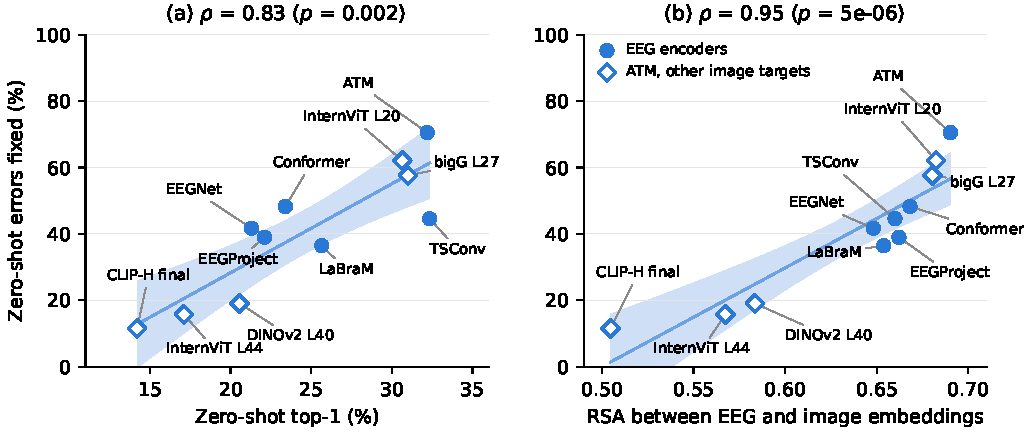
\includegraphics[width=\textwidth]{figures/encoders.pdf}
  \caption{Which encoders benefit from calibration. (a) Zero-shot accuracy against the fraction of zero-shot errors fixed by SAGE, for the ten encoders of Table~\ref{tab:encoders}. (b) The same fraction against RSA, for the ten encoders, 14 training variants of ATM-128 (image target, number of source subjects and of training concepts) and ATM-128 trained with an RSA loss. (c) Top-1 of ATM-128 against the InternViT-6B layer used as target. Variants use folds 1, 3 and 8; $\rho$ is Spearman's correlation.}
  \label{fig:encoders}
\end{figure*}

To assess the robustness of our framework, we evaluate SAGE across a diverse set of EEG encoder architectures (Table~\ref{tab:encoders}) and image targets (Fig.~\ref{fig:encoders}). We observe a notable reversal in architecture ranking: Squeezeformer is the strongest zero-shot encoder (36.5\%) but reaches 67.9\% after SAGE, while ATM-512, 6.4 points below it in zero-shot accuracy, reaches 78.7\%. SAGE fixes 46\% to 76\% of the zero-shot errors of the ten encoders, and zero-shot accuracy does not predict this fraction ($\rho=0.04$, $p=0.91$; Fig.~\ref{fig:encoders}a): it is 49\% for Squeezeformer and 76\% for ATM-128, at the same zero-shot accuracy. The representational similarity (RSA)~\cite{kriegeskorte2008rsa} between the two modalities predicts it ($\rho=0.92$, $p<0.001$; Fig.~\ref{fig:encoders}b). We compute RSA as the correlation between the pairwise cosine similarities of the centered test EEG embeddings and those of their images; it is invariant to rotations of either space and measures how well one orthogonal map, the one SAGE estimates, can superpose the two point clouds. RSA requires the true pairs, so it is a diagnostic for labeled source subjects; the label-free statistics we tried, including a Gromov--Wasserstein discrepancy~\cite{alvarezmelis2018gromov}, do not predict the gain.

\paragraph{Image targets and source subjects.}
The relation holds across 14 training variants of ATM-128 ($\rho=0.85$ with the encoders). The image target matters most: intermediate layers of InternViT-6B, OpenCLIP bigG~\cite{cherti2023openclip}, EVA02-E~\cite{fang2023eva02} and DINOv2~\cite{oquab2024dinov2} lead to 63\% to 83\% of the errors fixed, the final or near-final layers of CLIP ViT-H~\cite{radford2021clip}, InternViT-6B and DINOv2 to 17\% to 26\%, with a margin of SAGE over SCORE of 1 to 3 points instead of 13 to 17. Accuracy after calibration peaks at InternViT layers 28 and 31 (Fig.~\ref{fig:encoders}c), and the contrast between layers 28 and 44 holds for TSConv (38\% vs 10\% of the errors fixed). With 3 of the 9 source subjects, SAGE fixes 28\% of the errors, against 49\% with all 9 subjects and the same amount of training data (a third of the training concepts); from 6 subjects on, the number of subjects no longer matters at equal data.

\paragraph{RSA is not a training objective.}
Adding $1-\mathrm{RSA}$, computed on each batch, to the training loss of ATM-128 raises RSA from 0.70 to 0.77 but leaves SAGE at 89.0\% (crosses in Fig.~\ref{fig:encoders}b), and a five times larger weight lowers it to 84.0\%. The loss reaches a higher RSA by collapsing the EEG embeddings: their participation ratio, an effective number of dimensions, falls from 14.3 to 6.9, below the 11 to 19 of every other variant, and a rotation fitted on 100 labeled test pairs retrieves the other 100 with 49.5\% accuracy instead of 67.0\%. Across the other variants, this split-half rotation predicts the fraction of errors fixed as well as RSA does ($\rho=0.96$ vs 0.94). Training on it directly, with a loss that fits a rotation between two source subjects on half of the shared images of a batch and scores it on the other half, fails in the same way and more severely: the participation ratio falls to 1.8 and SAGE to 72.3\%. A penalty that keeps the participation ratio above 14 limits the collapse (9.5) and recovers part of the loss (85.5\%), still below the base encoder. RSA identifies a suitable geometry; optimizing it directly trades the instance-level information that the calibration needs for a global agreement it can already exploit.

\subsection{Streaming (R2)}
\label{sec:stream}

In R2, queries are drawn from a random menu of $K \in \{25, 50, 100, 150, 200\}$ images, averaged over $q \in \{5, 10, 20, 40\}$ repetitions, and arrive in random order; the calibration is re-fitted at 25 checkpoints, and results are averaged over three orders. Table~\ref{tab:stream} shows that undamped SAGE is harmful at the start of the stream: after the first refit, it decodes 17.9\% of the buffer correctly, against 39.5\% for the zero-shot decoder. On the intra-subject model, the harm dominates the whole stream, and the prequential accuracy of undamped SAGE is 5.4 points below zero-shot (0/10 subjects improved). The damping of Sec.~\ref{sec:method} removes the cold start in every setting we tested, with the constant fixed beforehand: the first refit is at the level of the zero-shot decoder, the final accuracy is unchanged, and the prequential accuracy improves over zero-shot by 23.2 points on ATM-128, 11.9 on TSConv and 5.1 intra-subject (10/10 subjects in each case, $p=0.002$). Damping the rotation alone is not sufficient (Table~\ref{tab:stream}), since whitening and CSLS are themselves poorly estimated on a small buffer. The gain is smallest when weak queries meet a large menu: with 50 refits, prequential accuracy improves by 14.1 points at $q=5$ and $K=200$ (32.6\% vs 18.5\%), against 22.5 points at $q=5$ and $K=25$.

\paragraph{SCORE in streams.}
With 50 refits and the three ATM-128 seeds, damped SAGE reaches a prequential accuracy of 62.4\%, against 56.4\% for SCORE re-fitted on the same buffers, which is better only on short buffers. Decoding with SCORE until the buffer holds 1.5 trials per menu item and with SAGE afterwards gives 63.5\%, and is at or above SCORE for all 20 combinations of menu size and repetitions. This switching point, selected leave-one-subject-out, is 1.5 in every fold.

\begin{table}[t]
\caption{Streaming (R2): prequential top-1 (each trial decoded on arrival), top-1 on the buffer after the first refit, and at the end of the stream.}
\label{tab:stream}
\centering
\small
\setlength{\tabcolsep}{3.4pt}
\begin{tabular}{@{}lcccccc@{}}
\toprule
 & \multicolumn{3}{c}{ATM-128} & \multicolumn{3}{c}{TSConv} \\
\cmidrule(lr){2-4}\cmidrule(lr){5-7}
Method & Preq. & First & End & Preq. & First & End \\
\midrule
Zero-shot & 39.8 & 39.5 & 39.8 & 36.2 & 34.7 & 36.2 \\
SAGE, undamped & 58.4 & 17.9 & \textbf{78.2} & 43.8 & 13.4 & 58.3 \\
rotation damped & 62.0 & 36.8 & 77.6 & 46.6 & 27.6 & 58.7 \\
SAGE (damped) & \textbf{63.0} & \textbf{41.5} & 77.6 & \textbf{48.0} & \textbf{34.6} & \textbf{58.9} \\
\bottomrule
\end{tabular}
\end{table}

\subsection{Coverage and Open Galleries (R3, R4)}
\label{sec:regimes}

Figure~\ref{fig:regimes} breaks the bijection. When only $U$ of the 200 concepts are queried, SAGE falls below the zero-shot decoder for $U \leq 75$ (10.3\% vs 26.8\% at $U=25$, all subjects harmed) and only overtakes SCORE at full coverage. When distractor images are added to the gallery, SAGE drops below SCORE from $D=200$ and to the level of the zero-shot decoder at $D=800$. The intra-subject model, whose zero-shot accuracy is 87.8\%, shows the same pattern (42.8\% vs 72.2\% for SCORE at $D=1{,}654$), so the failure is not a weakness of the base model but a wrong prior: balanced transport forces mass onto images that are not present. Restricting SAGE to the true set of present images restores its R1 accuracy at every $D$, which locates the problem in support estimation. Relaxing the column marginal~\cite{chizat2018scaling} reduces the harm without removing it (17.4\% at $U=25$, 14.3\% at $D=1{,}654$).

\paragraph{Support estimation.}
We select candidates from SCORE's scores, which involve no transport prior, and run SAGE on them only. With distractors, every query shows a different image, and a rectangular Hungarian assignment of the queries to the $200+D$ candidates selects 200 of them; in R1, it selects the whole gallery. Under partial coverage, queries repeat, so we keep the candidates that are the top-1 match of a query and replace the balanced plan by a row-wise softmax. With distractors, SAGE then matches or exceeds SCORE at every $D$ (56.2\% vs 53.6\% at $D=200$, 27.4\% vs 27.3\% at $D=1{,}654$) and keeps its 18-point lead at $D=0$. Under partial coverage, it is 1.2 points below SCORE at $U=25$ and above it from $U=100$ (Fig.~\ref{fig:regimes}, dashed). Which estimate applies depends on whether stimuli repeat, which the protocol knows; label-free statistics of the score matrix do not separate the regimes reliably, so the regime should be declared.

\begin{figure}[t]
  \centering
  \includegraphics[width=\columnwidth]{figures/regimes.pdf}
  \caption{Breaking the bijection (ATM-128, three seeds, 10 subjects, 3 draws). (a) R3: $U$ of the 200 concepts are queried, each one to four times, with 10-repetition queries. (b) R4: $D$ distractor images are added to the 200 candidates, with 80-repetition queries. SAGE + support restricts SAGE to a label-free estimate of the candidates present (Sec.~\ref{sec:regimes}). SCORE (original) uses SAMGA trained with SCORE's objective.}
  \label{fig:regimes}
\end{figure}

\subsection{How Many Labels Is Unlabeled Calibration Worth?}
\label{sec:labels}

We fit a supervised orthogonal map on $n$ labeled pairs of the target subject, taken from its training session (4-repetition averages of concepts disjoint from the test set), and score it with CSLS like SAGE. On ATM-128, the supervised map reaches 25.4\%, 52.1\%, 71.6\%, 78.7\% and 81.0\% for $n$ = 50, 200, 1{,}000, 5{,}000 and all 16{,}540 pairs, while unlabeled SAGE reaches 82.3\% from the 200 test queries alone ($+1.3$ over the full labeled session, $p=0.34$). The two are complementary: applying SAGE after the supervised map gives 93.0\% (10/10 subjects improved). On TSConv, labels are worth more: the supervised map overtakes SAGE between 1{,}000 and 5{,}000 pairs (74.0\% with all pairs vs 67.7\%), consistent with a smaller initial separation of true pairs in its embedding space (Sec.~\ref{sec:analysis}).

\subsection{What the Calibration Exploits}
\label{sec:analysis}

\paragraph{Signal-to-noise ratio.}
The gain of SAGE over zero-shot grows monotonically with the number of averaged repetitions per query: $-0.3$ at $q=1$, $+6.1$ at $q=5$, $+15.1$ at $q=10$, $+29.0$ at $q=20$ and $+47.1$ at $q=80$ on ATM-128. SAGE ties SCORE up to $q=5$ and its margin grows with $q$ (16.7 points at $q=80$). Across subjects, by contrast, the gain is not larger for weaker decoders (Spearman $\rho=-0.13$, $p=0.28$, within models). The calibration refines the initial predictions using the geometry of the task at hand, but cannot learn an efficient structure when the base predictions are noisy: it amplifies the signal present in the embeddings and does not compensate for its absence.

\paragraph{Geometry.}
On ATM-128, the median principal angle of the estimated rotation is 72$^\circ$, far from a small correction. The mean margin between the cosine of a query to its true image and its mean cosine to the other 199 images grows from 0.33 to 0.54, and the skewness of the hub-occurrence distribution drops from 2.27 to 1.05.

\paragraph{Sessions.}
The 80 test repetitions span four sessions. Calibrating on 20 repetitions of one session gives 56.0\%, against 52.7\% for a calibration fitted on another session and applied frozen (zero-shot 28.6\%; 9/10 subjects, $p=0.004$): 88\% of the gain carries over to a new session.

\paragraph{Normalization-based adaptation.}
AdaBN adds 2.7 points to the zero-shot ATM-128 decoder but nothing after SAGE, and degrades TSConv after SAGE ($-6.8$); TENT adds nothing to AdaBN.

%=====================================================================
\section{Pitfalls}
\label{sec:pitfalls}

\begin{table*}[t]
\caption{Eight pitfalls of transductive calibration, quantified on our pipeline (ATM-128 unless stated).}
\label{tab:pitfalls}
\centering
\small
\setlength{\tabcolsep}{4pt}
\begin{tabular}{@{}llp{7.6cm}l@{}}
\toprule
 & Pitfall (assumption) & Effect on our pipeline & Remedy \\
\midrule
P1 & Checkpoint selected on the target subject (A3) & zero-shot $+2.7$ (36.0 vs 33.4); SAGE $-1.9$ (82.3 vs 84.2) & validation split \\
P2 & Calibration tuned on the target subject (A3) & $+3.9$ (86.2 vs 82.3); label-free rules: 41.4 on TSConv & cross-fold selection \\
P3 & Bijection assumed under partial coverage (A2) & $U=25$: $-16.5$ vs zero-shot, 10/10 subjects harmed & declare the regime \\
P4 & Closed gallery assumed with distractors (A2) & $D=1{,}654$: $-2.0$ vs zero-shot, $-15.5$ vs SCORE & estimate the support \\
P5 & Gains compared at different query SNR (A4) & gain over zero-shot $+15.1$ at $q=10$ vs $+47.1$ at $q=80$ & report $q$ \\
P6 & Batch size assumed large (A1) & first stream refit 17.9 vs 39.5 zero-shot (intra: 29.7 vs 82.2) & damping \\
P7 & Mean-only reporting & $D=800$: mean $0.0$, but 4/10 subjects lose, up to $-9.3$ & per-subject, harm rate \\
P8 & Prior credited to the calibration (A2) & one-to-one decoding alone: 66.2; SCORE: 66.5 & prior-only control \\
\bottomrule
\end{tabular}
\end{table*}

Table~\ref{tab:pitfalls} quantifies eight pitfalls on our own pipeline, each tied to one of the assumptions of Sec.~\ref{sec:setting}. Choosing the checkpoint on the test subject (P1), as all compared work does, inflates zero-shot accuracy by 2.7 points on a model trained with a held-out validation split of 10\% of the training concepts, but not the calibrated accuracy, which is 1.9 points \emph{higher} with the clean checkpoint. Tuning calibration hyper-parameters on the test subject (P2) inflates SAGE by 3.9 points, and label-free selection rules computed on the target batch are unreliable. The mean hides harm (P7): at $D=800$, SAGE and the zero-shot decoder are equal on average, while four subjects lose up to 9.3 points.

%=====================================================================
\section{Discussion and Conclusion}
\label{sec:discussion}

\paragraph{Evaluation benchmarks and community standards.}
We have followed the model selection protocol used throughout this literature~\cite{zhang2025neurobridge,du2025shallow,huang2026sattc} to ensure fair comparison with prior work. However, this selection protocol, while appropriate for the structure of the THINGS-EEG-2 dataset, which does not natively offer a validation set, is a form of information leakage: the held-out subject is implicitly used for model selection. Our results show that it matters less after calibration than before (P1), and less than leakage in the calibration hyper-parameters (P2). We encourage future work in this area to adopt a validation split or an equivalent clean evaluation as a primary reported metric. The standard 200-way test is also a bijection, so a calibration evaluated only on it may be measuring the correspondence prior; we encourage future work to report the prior-only control, the number of averaged repetitions, per-subject results, and at least one regime beyond the bijection. More broadly, the field would strongly benefit from the development of additional visual decoding benchmarks. Most previous studies have evaluated their methods exclusively on THINGS-EEG-2, which raises concerns about dataset-specific conclusions. \TODO{Alljoined-1.6M and THINGS-MEG results.} Broader community efforts toward standardized multi-dataset benchmarks will be essential for establishing reliable comparisons and accelerating progress in visual neural decoding.

\paragraph{Limitations and future work.}
SAGE benefits from a one-to-one matching structure and degrades when it is absent. Our label-free support estimates bring it back to the level of SCORE, not beyond: with 1{,}654 distractors, knowing the support would still add 57 points. Support estimation, \ie deciding without labels which candidates are present, remains the open problem. The gain is also smallest for weak queries against a large menu (Sec.~\ref{sec:stream}), where the encoder leaves too little structure to refine. Our streams are offline replays of a rapid serial visual presentation paradigm from 10 subjects, with queries averaging repeated presentations of one exemplar per concept. While realistic closed-loop BCI settings~\cite{lawhern2018eegnet} may require sequential adaptation, transductive calibration remains applicable in constrained regimes where the candidate pool is known, such as closed-menu or shortlist-based assistive interfaces, and reranking settings in which an inductive base decoder first narrows the candidate pool. More generally, many BCI systems operate within a task-dependent context: if the user is working in a spreadsheet, the relevant vocabulary may be actions such as copy, paste, or sort, whereas in an image-editing application it may instead be brush, erase or zoom. In such cases, one can maintain a context-dependent bank of plausible actions and perform set-level calibration within that restricted pool. Neither SAGE nor the protocol is specific to EEG: the calibration acts on embeddings and is indifferent to their origin, and measuring it on fMRI and MEG retrieval pipelines~\cite{scotti2024mindeye2,hebart2025thingsmeg} is a natural next step. Finally, the fact that an orthogonal alignment estimated from unlabeled data recovers a large part of the accuracy lost on a new subject motivates lighter-weight subject adaptation, geometrically motivated few-shot calibration, and inductive approaches that recover a corrective structure without access to the full test set.

\paragraph{Conclusion.}
We formalized label-free transductive subject calibration for EEG-to-image decoding, made explicit the assumptions under which it is evaluated, and introduced SAGE. The zero-shot encoder alone is our claim about cross-subject decoding in general; in the transductive setting, where the unlabeled queries of the new subject and the candidate set are processed jointly, SAGE raises cross-subject top-1 accuracy on THINGS-EEG-2 from 35.8\% to 84.6\%. Taken together, these results show that a corrective orthogonal transformation estimated from unlabeled data recovers a large part of the cross-subject accuracy gap, to the extent that the similarity structure of the EEG embeddings follows that of the image targets, and that this estimate relies on the structure of the test set, which evaluations of calibration methods should make explicit.

\section*{LLM Usage Statement}
\TODO{Draft, to be checked and completed by the authors.} Claude (Anthropic) was used as a coding agent: it wrote and ran part of the experiment code (training and evaluation scripts, the analyses of Secs.~\ref{sec:regimes} and~\ref{sec:encoders}), produced the figures, and drafted and edited parts of the text.

{
    \small
    \bibliographystyle{ieeenat_fullname}
    \bibliography{references}
}

\end{document}
